\documentclass[10pt, conference, compsocconf]{IEEEtran}

\usepackage{capt-of}
\usepackage{graphicx}
\usepackage{subfig}
\usepackage{booktabs}
\usepackage{multirow}
\usepackage{siunitx}
\usepackage{multicol}
\usepackage{array}
\usepackage{amsmath}
\newcommand{\nltable}[2][c]{%
  \begin{tabular}[#1]{@{}c@{}}#2\end{tabular}}
\newcommand{\wave}{\raise.17ex\hbox{$\scriptstyle\mathtt{\sim}$}}

\newcolumntype{C}[1]{>{\centering\let\newline\\\arraybackslash}m{#1}}

\begin{document}
\bstctlcite{IEEEexample:BSTcontrol}

\title{Approach of Matrix Multiplication on Cloud Distributed System}


\author{\IEEEauthorblockN{Myungjun Son}
\IEEEauthorblockA{Department of Computer Science\\
Kookmin University\\
Seoul, South Korea\\
smj8612@kookmin.ac.kr}
\and
\IEEEauthorblockN{Kyungyong Lee}
\IEEEauthorblockA{Department of Computer Science\\
Kookmin University\\
Seoul, South Korea\\
leeky@kookmin.ac.kr}
}

% make the title area
\maketitle

\begin{abstract}
Abstract
\end{abstract}

\IEEEpeerreviewmaketitle

\section{Introduction}\label{sec:intro}
Big data analytics systems are deployed in cloud computing environments to process ever-increasing dataset while guaranteeing stable operations; scalability and fault-tolerance from the perspective of infrastructure. To satisfy application demands from distinct use cases, cloud computing service providers offer various types of instances that applications can run. Using those resources, most big data platforms are deployed in a scale-out manner. As managing distributed datasets and tasks running on large-scale machines are challenging, abstractions of distributed datasets and resources are crucial to let application developers focus on tasks that really matter. Many systems are proposed to provide a simple and easy interface to handle large-scale datasets, to name a few, Hadoop~\cite{hadoop}, Spark~\cite{spark}, and recently TensorFlow~\cite{tensorflow}.

To extract valuable insights from massive dataset, matrix multiplication is widely used. In recommendation systems, for example, the core computation kernel of matrix factorization algorithms, such as SVD and NMF~\cite{nmf}, is matrix-matrix multiplication. The matrix-vector multiplication is the core kernel in page-rank algorithm when using the power method to get principle eigen vectors~\cite{pagerank}. In order to build a cost efficient cloud environment that runs data mining tasks with distributed matrix computation kernel, it is crucial to estimate the kernel task overhead on different cloud computing instances with distinct matrix size. 

To understand the characteristics of matrix multiplication performance on a distributed cloud computing environment, we analyzed the performance of dense matrix multiplication with diverse input sizes and formations on distinct cloud computing instances. In the experiments, we multiply two square matricies with the number of rows being 10000, 20000, and 30000 on AWS EC2 \textit{R4, T2, M4, C4, G2} instances with size of \textit{2xlarge}. We use Apach Spark MLLib BlockMatrix library~\cite{spark-mm} to conduct the experiments with four machines that have OpenBlas installed. 

Figure~\ref{fig:different-instance-types} shows the normalized latency to the fastest completing instance type in the gray bar. As shown in the figure, as the input matrix size differs, the best performing instance type also differs - no globally optimal instance type. If we consider the price factor of each instance, the performance difference even gets bigger as shown in the red star mark. Furthermore, as shown in the Figure~\ref{fig:instance-blocks-sizes-compare}, multiplying two non-sqaure matricies shows siginificantly different performance comparing to the square matrix multiplication though the number of compute operation is the same - i.e., the number of (left matrix rows $\times$ left matrix columns $\times$ right matrix columns).

\begin{figure}[!ht]
  \centering
  \subfloat[Performance of different instance types of 2xlarge]{\label{fig:different-instance-types}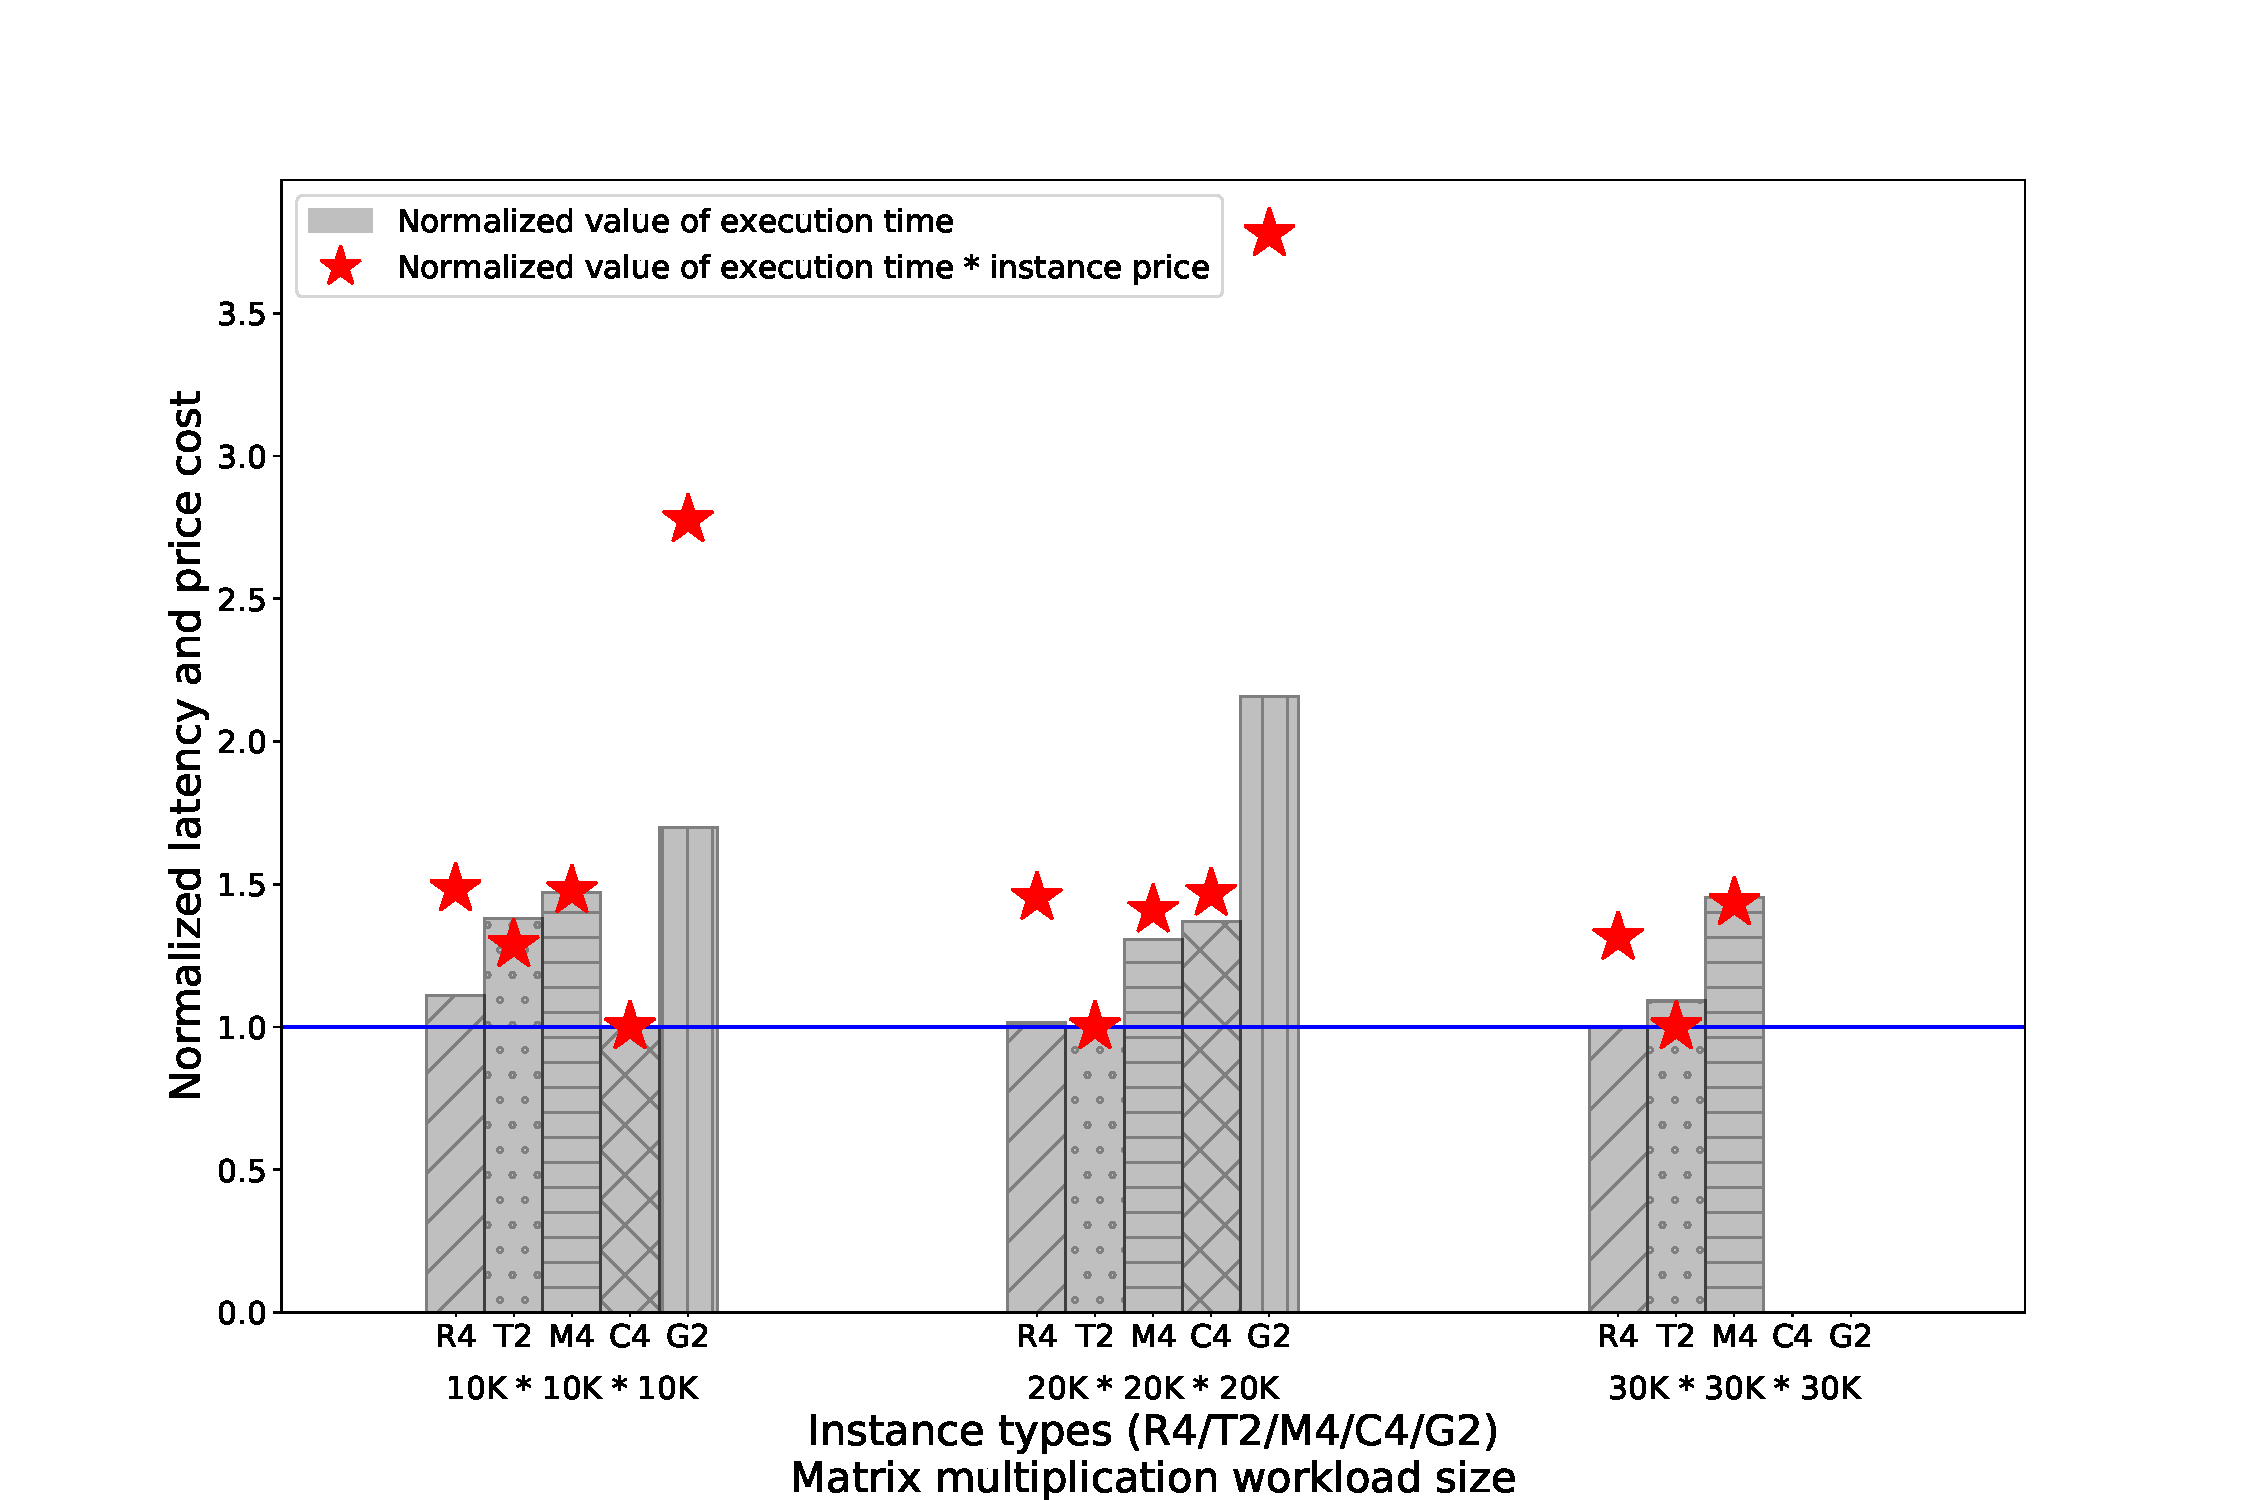
\includegraphics[width=0.5\textwidth]{figures/instance-2xl-compare.pdf}}\\
  \subfloat[Performance of different matrix shapes]{\label{fig:different-matrix-shapes}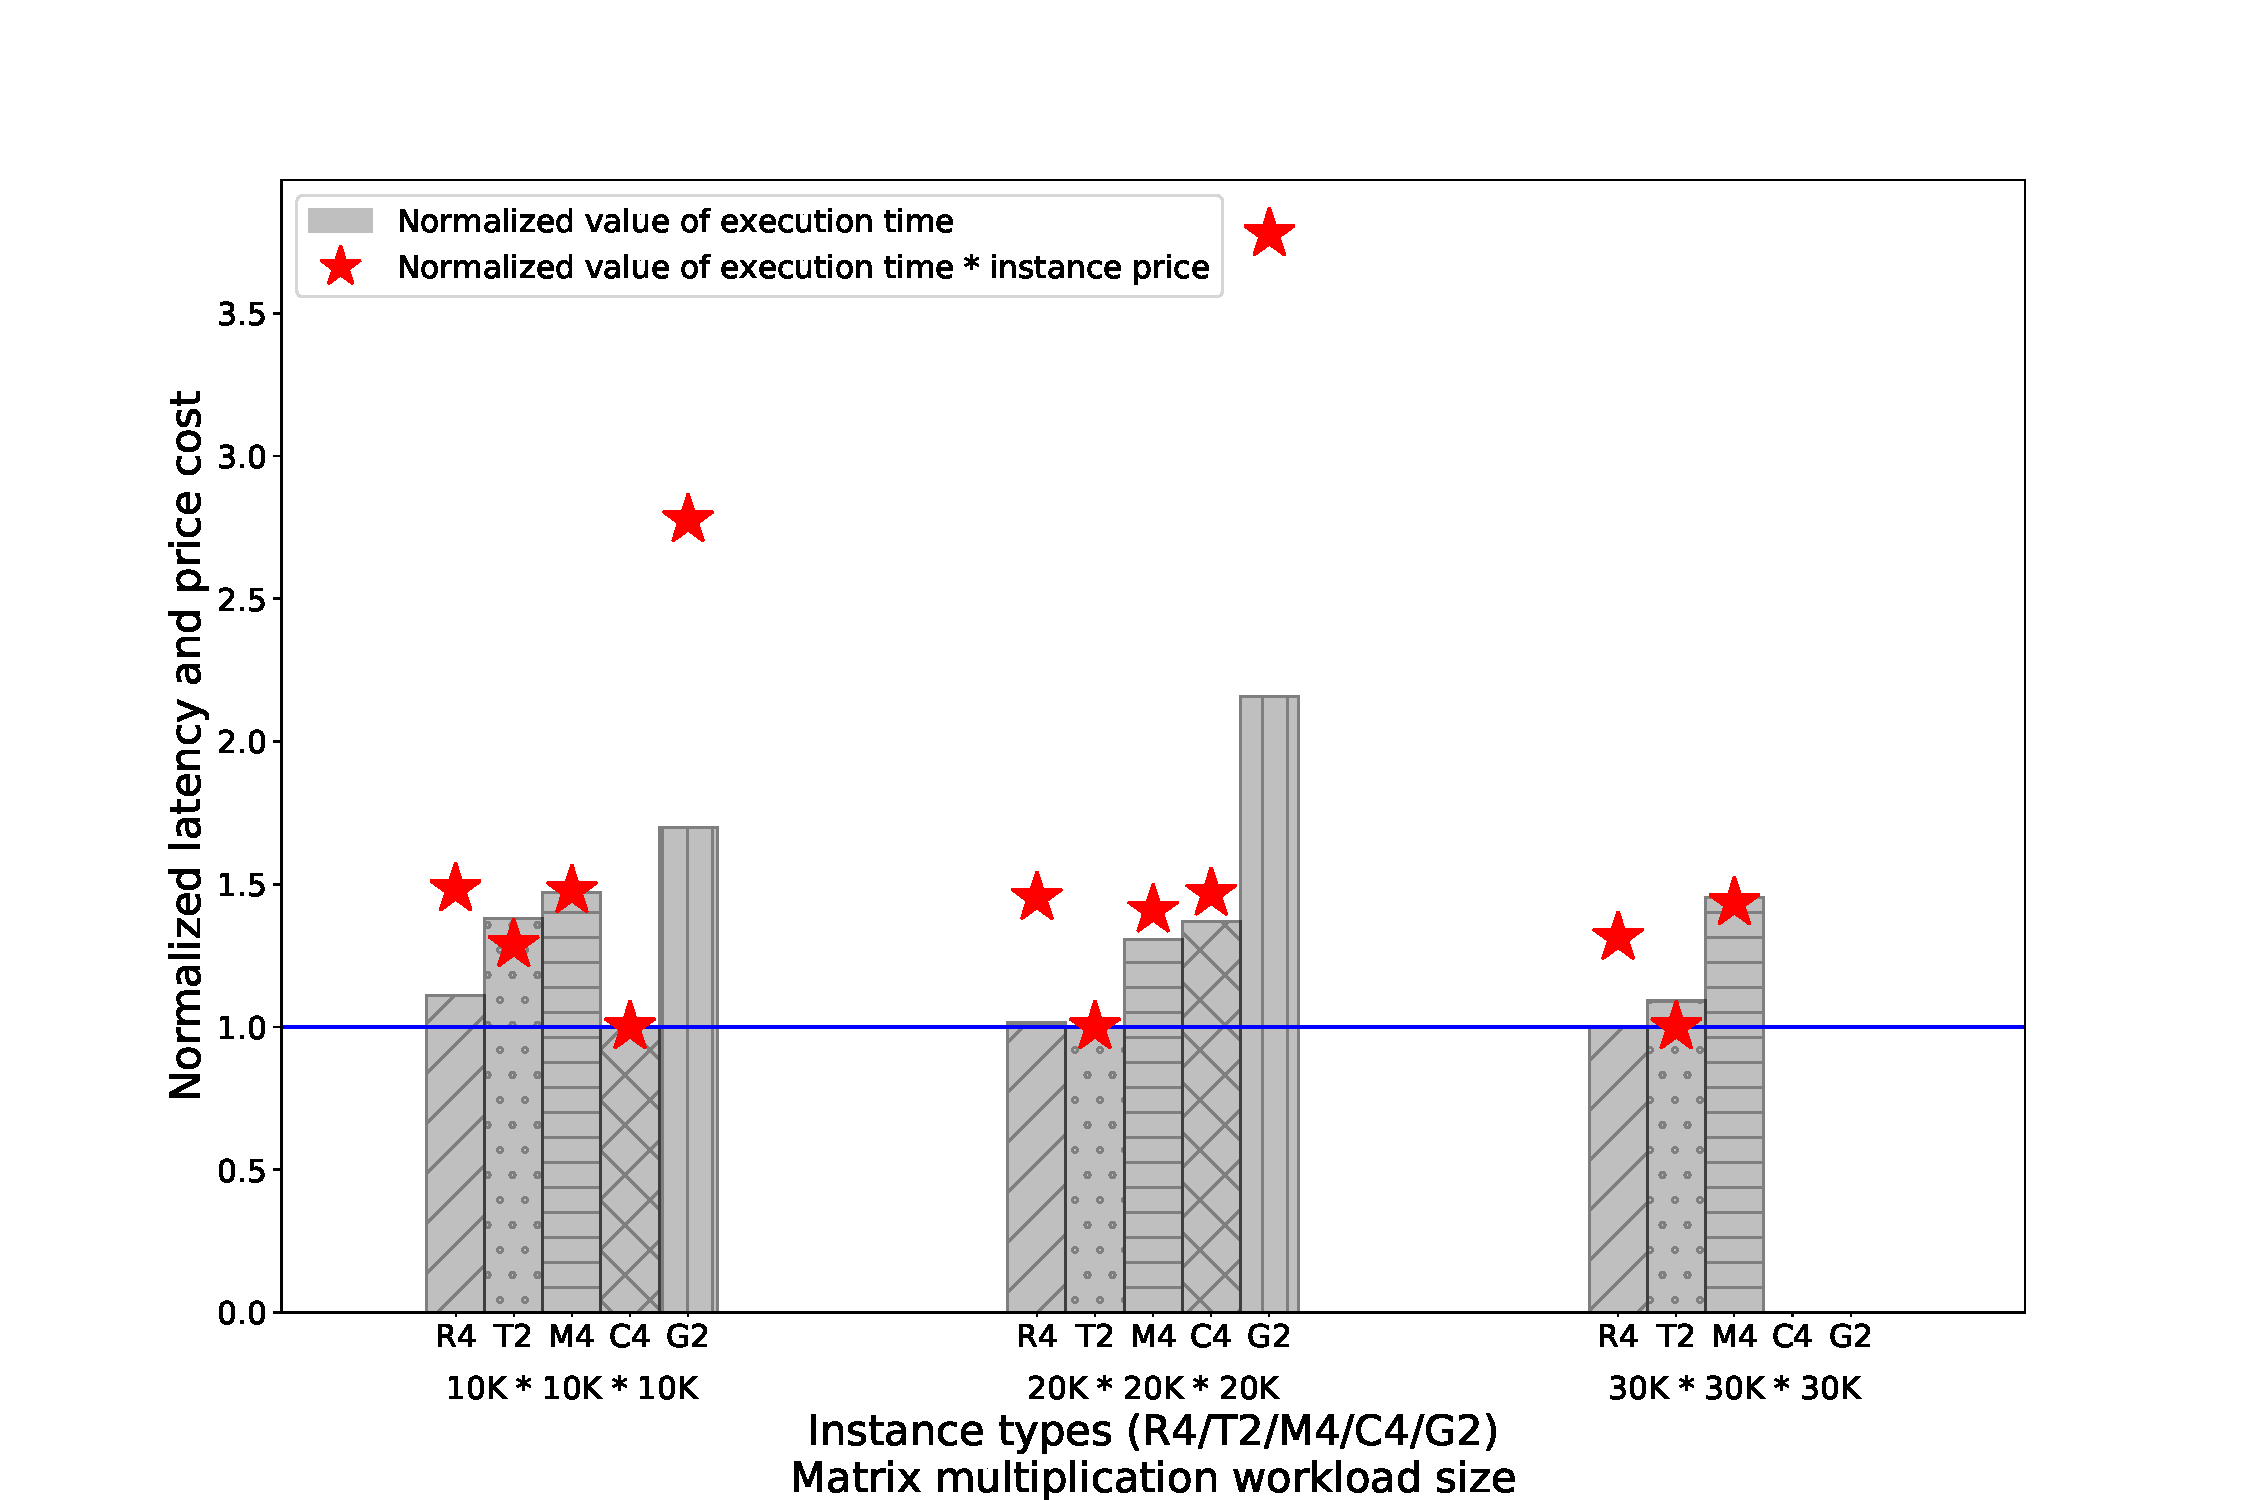
\includegraphics[width=0.5\textwidth]{figures/instance-2xl-compare.pdf}}
  \caption{\label{fig:instance-blocks-sizes-compare}. The normalized value of latency with respect to different instance types and input matrix shapes - the lower, the better.}
\end{figure}

Despite of the importance of the matrix multiplication when running machine learning tasks, performance analysis and modeling in a distributed cloud computing environment are not thoroughly conducted yet. Few works focused on predicting data mining algorithm performance on a cloud comptuing environment - Ernest~\cite{ernest}, CherryPick~\cite{cherrypick}, and PARIS~\cite{paris}. The proposed methods rely on a scale-based sampling method to estimate the latency to complete original large input size, and they show poor accuracy when predicting distributed matrix multiplication task running time as they fail to catpture the nature of distrbuted matrix computation. Performance modeling and prediction on a single machine with multiple cores are well studied in literature with hardware optimized libraries, such as OpenBLAS, but previous works generally do not consider network and IO overhead that can be additional significant overhead in a distributed cloud computing environment.

In this paper, we propose MPC (\textbf{M}atrix Multiplication \textbf{P}erformance Predictor for \textbf{C}loud Computing) to provide accurate latency prediction while performing multiplication of arbitrary shape and size of matricies on diverse cloud computing resources. MPC profiles the latency to perform multiplication on two unit-block matricies on diverse cloud computing resources. In order to represent the profiled unit-block latency results, MPC builds a model with XXXX followed by bayesian optimization to find the optimal hyper parameters to minimize the modeling error. In the step of prediction of arbitrary size matrix multiplication, MPC proposes to disassemble the input matricies into blocks that worker nodes can operate, and the latency to multiply each block matrix is made by using the model built from the unit-block matricies. MPC eventually stitches the blocks to conjecture the overall task completion time.

% summarize the result
% itemize the contributions

\section{Matrix Multiplication on a Distributed Computing Environment}\label{sec:distributed-matrix-computation}
% explain how the matrix computation happens in spark - mention the step of shuffle, compute, reduce
% How block matrix multiplication happens with the overhead (shuffle, compute, reduce)
Optimization of distributed matrix multiplication is well studied in literature. In the HPC community, many works focused on minimzing communication cost using MPI model. Representative works include SUMMA~\cite{summa} and CARMA~\cite{carma}. Despite of the performance optimality of the methods, they have limitations regarding the programmability, scalability, and robustness comparing to general purpose big-data analytics systems, such as Spark~\cite{spark} and Hadoop~\cite{hadoop}, especially on a shared cloud computing environment.

Apache Spark is an open source big-data analytics platform. The primary abstraction in Spark is Resilient Distributed Dataset(RDD), which represents a read-only collection of objects partitioned across a set of machines. Spark manages large-scale data using partitions that helps parallelize distributed data processing while guaranteeing the fault-tolerance with lineage and task execution optimization with lazy evaluation~\cite{spark}.

In Spark, matrix-related linear algebric operations are supported in the MLLib library~\cite{spark-mm} with various matrix partitioning heuristics (row-, column-, and block-based) and a set of distributed operation APIs on the matrix. To multiply two matricies, Spark MLLib automatically identifies the optimal way of task distribution based on the input matrix partitioning scheme and uses Scala Breeze library to execute multiplication. Let us give an example of multiplying two matricies, $C = A \times B$. If $A$ is row-partitioned and $B$ is column-partitioned, the cartesian product is performed for each row block of $A$ and column block of $B$. If both $A$ and $B$ are block-partitioned, the block dimension of result matrix, $C$, is decided by considering the number of workers and input block dimensions. A work node that is responsible for each resulting block fetches all the necessary blocks from $A$ and $B$ to execute multiply operation locally.

% Add a figure to explain the matrix multiplication of block-based

Figure~\ref{fig:matmul-with-overhead} shows an example of block-based matrix multiplication. A left matrix, $A$, is block-partitioned by $2 \times 3$, a right matrix, $B$, is partitioned by $3 \times 2$, and the result matrix, $C$, is partitioned by $2 \times 2$. In Spark, a \textit{cogroup} operation by the result matrix block index allows a worker node that is responsible for a result block to collect necessary left and right matrix blocks. During \textit{cogroup} operation, network overhead is dominant. After collecting all necessary blocks, each worker node performs a product operation followed by an element-wise addition. In the step, I/O overhead to read the fetched blocks from a \textit{local.dir} location and compute overhead dominates.

\subsection{Matrix Multiplication Overhead Modeling}

\section{Evaluation}{\label{eval}}

\section{Related Work}\label{sec:relatedwork}
\textbf{Instance Recommendation:} Ernest~\cite{ernest} predicts performance for different VM and cluster sizes, targeting machine learning analytics applications. PARIS~\cite{Yadwadkar:2017:SBV:3127479.3131614} takes a hybrid online/offline approach, using a random forest model to predict application performance on various VM configurations based on features such as CPU utilization obtained from profiling. None of these systems consider the I/O overhead modeling in distributed cloud environments with arbitrary matrix shape which can affect matrix computation performance. 

%need taming
\textbf{Analyzing performance of data analytics frameworks:} While previous studies have analyzed how CPU, memory, network and storage resources affect Spark performance ~\cite{196352,li2014tachyon,ousterhout2015making} our work is the first to take consideration that I/O overhead can affect shape of the matrix. 

% need taming
% cloud computing performance prediction
% instance recommendation (Ernest, Paris, CCGrid 2017)
% Matrix multiplication performance and Spark + Matrix multiplication

\section{Conclusion and Future Work}
Conclusion~\cite{tr-spark}


\bibliographystyle{IEEEtranS}
\bibliography{abc2}
\end{document}
